\subsection{De la présence à l'apprentissage : incarnation et agence sociale}
\label{subsec:incarnation_agence_sociale}

La théorie de l'agence sociale formalise le lien entre présence sociale et apprentissage. Le modèle, développé à partir d'expériences comparant des agents avec et sans indices sociaux, propose une chaîne causale en quatre maillons : les indices sociaux (voix, visage, gestes) activent la présence sociale, qui génère chez l'apprenant la perception d'un partenariat, laquelle augmente l'effort de traitement et améliore l'apprentissage en profondeur \citep{moreno2001-th, mayer2012}. Cette théorie se distingue de la CTML (cf.~\ref{subsec:architecture_cognitive}) sur un point essentiel : l'amélioration de l'apprentissage ne résulte pas d'une optimisation du traitement de l'information entre canaux cognitifs, mais d'une motivation sociale à traiter l'information plus profondément. L'apprenant fournit un effort supplémentaire non pas parce que l'information est mieux présentée, mais parce qu'il perçoit un interlocuteur qui mérite son attention.

Les agents pédagogiques se différencient selon quatre dimensions principales. Le tableau~\ref{tab:typologie_agents} présente cette classification.

\begin{table}[ht]
\centering
\caption{Typologie des agents pédagogiques}
\label{tab:typologie_agents}
\small
\begin{tabular}{p{2.8cm} p{10.5cm}}
\hline
\textbf{Dimension} & \textbf{Catégories} \\
\hline
Forme & Texte seul ; Voix seule ; Avatar 2D ; Avatar 3D ; Humain filmé \\
\hline
Rôle pédagogique & Instructeur (transmission directe) ; Tuteur (guidage individualisé) ; Compagnon (collaboration entre pairs) ; Motivateur (soutien affectif) \\
\hline
Anthropomorphisme & Faible (icône, robot stylisé) ; Moyen (avatar cartoon) ; Élevé (humanoïde réaliste) \\
\hline
Technologie & Scriptée (arbre de décision) ; Basée règles (système expert) ; NLP/ML (traitement du langage naturel) ; IA générative (LLM) \\
\hline
\end{tabular}
\end{table}

L'évolution des agents virtuels sur trois décennies illustre un déplacement progressif des priorités de conception. Les premiers systèmes, tel Gandalf développé pour la communication multimodale, établissaient les bases de l'interaction naturelle en combinant reconnaissance gestuelle, vocale et regard \citep{thorisson1997}. Les agents pédagogiques comme Steve ont ensuite transposé ces principes au domaine éducatif, démontrant que des avatars aux capacités graphiques limitées pouvaient activer les mécanismes de présence sociale décrits en section~\ref{subsec:presence_sociale_CASA} \citep{johnson2000}. La génération suivante s'est focalisée sur l'expressivité émotionnelle, avec des systèmes capables de générer des comportements affectifs cohérents à partir de modèles computationnels de l'émotion \citep{ochs2008}. Les agents contemporains intègrent ces acquis dans une architecture multimodale où voix, expressions faciales et comportements non verbaux interagissent pour construire la confiance et maintenir l'engagement \citep{torre2019}. La figure~\ref{fig:evolution_agents} illustre cette trajectoire sur près de vingt-cinq ans. Elle révèle un paradoxe : l'amélioration technique n'a pas résolu la question de l'efficacité pédagogique, qui dépend moins du réalisme visuel que de la cohérence des indices sociaux déployés.

\begin{figure}[ht]
\centering
\begin{subfigure}[b]{0.45\textwidth}
    
\includegraphics[width=\textwidth]{images/ch2/thorisson1996_gandalf.png}
    \caption{Gandalf \citep{thorisson1997}}
\end{subfigure}
\hfill
\begin{subfigure}[b]{0.45\textwidth}
    \includegraphics[width=\textwidth]{images/ch2/steve_johson1997.png}
    \caption{Steve \citep{johnson2000}}
\end{subfigure}
\vspace{0.5cm}
\begin{subfigure}[b]{0.45\textwidth}
    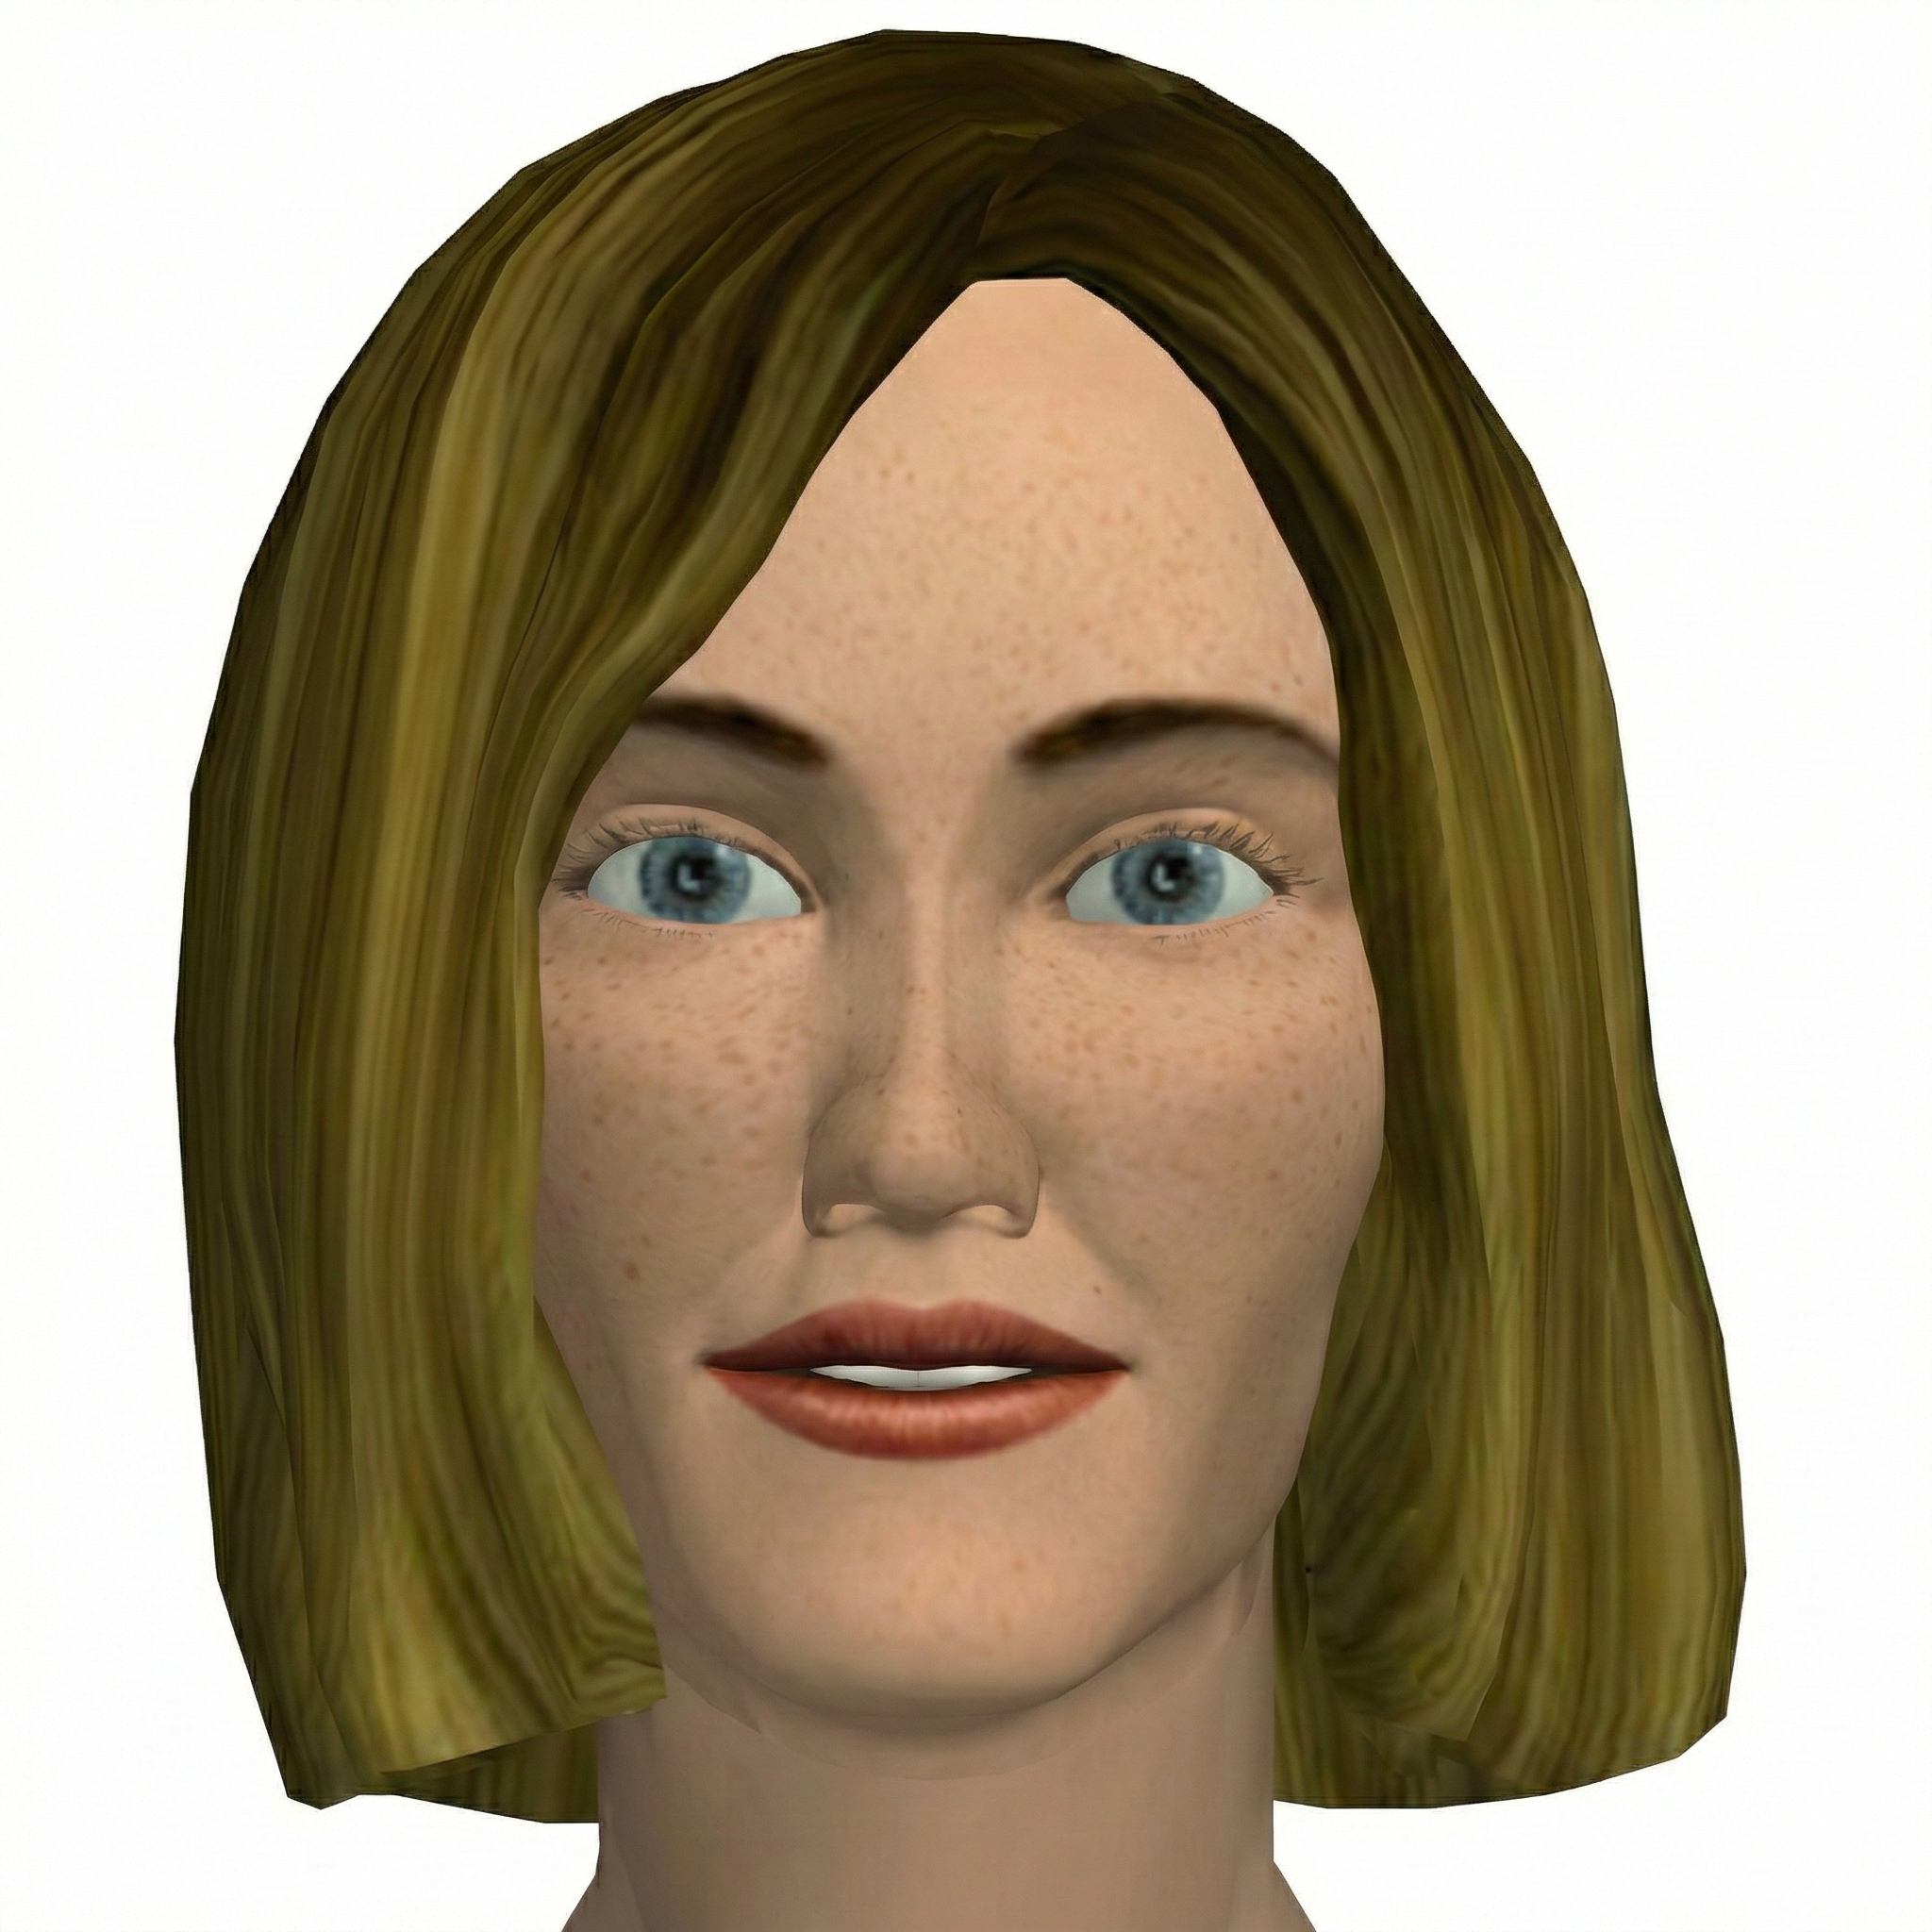
\includegraphics[width=\textwidth]{images/ch2/ochs2010.png}
    \caption{Agent expressif \citep{ochs2008}}
\end{subfigure}
\hfill
\begin{subfigure}[b]{0.45\textwidth}
    \includegraphics[width=\textwidth]{images/ch2/torre2019.png}
    \caption{Agent multimodal \citep{torre2019}}
\end{subfigure}
\caption{Évolution des agents virtuels sur trois décennies. De Gandalf (1996), premier système conversationnel multimodal, à Steve (2000), agent pédagogique pour l'entraînement naval, puis aux agents expressifs capables de modéliser des états émotionnels complexes (2008), jusqu'aux systèmes contemporains intégrant expression multimodale et confiance (2019).}
\label{fig:evolution_agents}
\end{figure}

Les signaux sociaux par lesquels un agent active la chaîne causale de l'agence sociale se répartissent en trois catégories. Le tableau~\ref{tab:signaux_sociaux} présente cette taxonomie, les mécanismes théoriques associés et les effets documentés.

\begin{table}[ht]
\centering
\caption{Taxonomie des signaux sociaux des agents pédagogiques}
\label{tab:signaux_sociaux}
\small
\begin{tabular}{p{1.8cm} p{3cm} p{4.5cm} p{4.5cm}}
\hline
\textbf{Catégorie} & \textbf{Signaux} & \textbf{Mécanisme} & \textbf{Effet documenté} \\
\hline
Vocaux & Voix humaine, prosodie, ton émotionnel & Perception d'un esprit (\textit{mind perception}) ; activation du canal auditif sans surcharge visuelle & Voix humaine > synthétique pour le transfert \citep{craig2017} ; indices vocaux > visuels pour la présence sociale \citep{ehret2021} \\
\hline
Visuels & Expressions faciales, gestes déictiques, regard, posture & Signalisation attentionnelle ; guidage de l'attention vers le contenu pertinent & Gestes déictiques améliorent le transfert proche \citep{davis2018} ; l'effet dépend du type d'apprentissage visé \citep{baylor2009} ; gestes même non liés au contenu améliorent rétention et transfert \citep{schneider2022} \\
\hline
Compor\-tementaux & Réactivité, feedback adaptatif, expressivité émotionnelle contextualisée & Contingence conversationnelle ; maintien du contrat social ; crédibilité par congruence émotionnelle & L'expressivité émotionnelle améliore le transfert \citep{wang2023-meta} ; chaleur et expressions émotionnelles renforcent la confiance \citep{sinatra2021} ; l'expressivité contextualisée augmente la crédibilité \citep{yanqing2023, oker2020} \\
\hline
\end{tabular}
\end{table}

Parmi ces signaux, la voix constitue l'indice social le plus robuste. La perception d'une voix humaine --- par opposition à un texte écrit --- suffit à déclencher l'attribution d'un esprit à l'agent : l'auditeur infère des intentions, des émotions et une capacité de compréhension \citep{schroeder2016}. En contexte d'apprentissage, la voix humaine produit de meilleurs résultats que la voix synthétique, un effet qui s'observe sur le transfert et la compréhension mais pas systématiquement sur la rétention factuelle \citep{craig2017}. La combinaison d'émotions positives et de caractéristiques vocales humaines renforce la motivation et les états affectifs des apprenants \citep{wang2021}, tandis que la fluence et la naturalité de l'interaction vocale contribuent à l'engagement conversationnel \citep{reicherts2022}. La prosodie --- variations de hauteur, de rythme et d'intensité --- contribue indépendamment de la qualité vocale : les indices prosodiques pèsent davantage que les indices visuels dans la construction du sentiment de présence sociale \citep{ehret2021}. Une voix synthétique au ton monotone peut ainsi annuler le bénéfice d'un visage expressif \citep{craig2019, chiou2020}. Des données récentes d'oculométrie confirment cette hiérarchie : la combinaison voix humaine et apparence formelle améliore l'apprentissage tout en réduisant la charge cognitive, et oriente l'attention vers le contenu plutôt que vers l'agent \citep{xiao2025}. La voix occupe donc le premier rang dans la hiérarchie des indices sociaux, ce qui a une implication directe pour le design : investir dans la qualité vocale produit un meilleur rendement que raffiner l'apparence visuelle.

L'incarnation visuelle --- la présence d'un corps ou d'un visage à l'écran --- produit des effets plus nuancés. La présence visuelle contribue à induire un sentiment de présence sociale qui renforce l'engagement émotionnel et la motivation \citep{sanghoon2015, alemdag2022-rc}, et l'apparence de l'agent influence la perception de compétence et l'attitude envers le contenu \citep{domagk2010}. La comparaison entre un agent visible et une narration seule (voix sans corps) montre un avantage pour l'agent incarné sur le transfert \citep{mayer2012}. Cet avantage n'est cependant pas universel : une revue systématique rapporte que la majorité des études examinées ne trouvent pas de différence d'apprentissage attribuable à la seule présence visuelle \citep{heidig2011}, et une revue des comportements non verbaux dans les agents virtuels confirme l'inconsistance des résultats \citep{wangruiz2021}.

Cette dissociation entre présence visuelle et apprentissage trouve une formulation théorique dans la distinction entre propriétés externes et internes des agents pédagogiques \citep{moreno2004}. Les propriétés externes --- image et voix --- constituent la persona de l'agent, tandis que les propriétés internes désignent les méthodes pédagogiques qu'il met en œuvre : feedback, guidage, modélisation. Les travaux conduits avec Herman The Bug, un personnage 2D fictionnel enseignant la botanique, ont permis d'isoler ces deux dimensions \citep{lester1999}. La présence visuelle de l'agent n'affecte pas l'apprentissage lorsque les méthodes pédagogiques restent constantes. L'image animée ne produit ni bénéfice ni interférence mesurable par rapport à une narration seule. Ce résultat, répliqué dans plusieurs contextes expérimentaux, suggère que l'effet d'agence sociale opère principalement par le canal auditif : la voix suffit à activer la perception d'un partenaire, l'image n'y ajoute qu'une contribution marginale.

Le regard de l'agent illustre cette ambiguïté. Le contact visuel direct augmente le temps de fixation oculaire sur l'agent, ce qui devrait favoriser l'apprentissage selon les modèles attentionnels. L'effet observé est inverse : le regard direct réduit la performance, un résultat interprété comme une surcharge du canal visuel --- l'apprenant consacre des ressources cognitives au traitement du regard au détriment du contenu \citep{wilson2018, wang2017}. La comparaison entre agents 2D et 3D révèle un paradoxe comparable : les agents en 2D produisent des résultats supérieurs à ceux des agents en 3D, ce qui indique que le réalisme géométrique ne détermine pas l'efficacité pédagogique \citep{castro-Alonso2021-qh}. L'efficacité des signaux visuels dépend en outre du type d'apprentissage visé : les gestes déictiques améliorent l'apprentissage procédural, tandis que les expressions faciales favorisent l'apprentissage attitudinal \citep{baylor2009}. Les gestes et expressions non directement liés au contenu améliorent néanmoins la rétention et le transfert tout en rendant l'agent plus humain, sans générer de surcharge cognitive \citep{schneider2022}.

Les méta-analyses convergent vers un portrait cohérent de l'efficacité des agents pédagogiques. L'expressivité émotionnelle améliore davantage le transfert que la rétention ou la motivation \citep{wang2023-meta}. Les gestes déictiques --- pointer vers un élément pertinent du contenu --- produisent l'effet le plus marqué parmi les signaux visuels \citep{davis2018}. Les agents intégrant des technologies d'intelligence artificielle obtiennent des résultats supérieurs aux agents scriptés \citep{dai2024-gv}. Les effets motivationnels présentent un profil distinctif : les agents améliorent l'auto-efficacité et l'intérêt, mais n'ont pas d'effet détectable sur la motivation intrinsèque \citep{gladstone2025}. Le tableau qui se dessine est celui d'un outil dont les bénéfices sont réels mais modestes, davantage orientés vers le traitement en profondeur que vers la mémorisation, et dont l'efficacité dépend moins du réalisme visuel que de la qualité des indices sociaux déployés.

Ces effets positifs se heurtent toutefois à un plafond structurel. Les agents classiques fonctionnent à partir de scripts prédéfinis : leurs réponses sont sélectionnées dans un arbre de décision, sans adaptation au contenu de l'échange en cours. Cette rigidité érode progressivement la présence sociale, car l'apprenant détecte l'absence de contingence --- l'agent ne répond pas véritablement à ce qui a été dit, il sélectionne une réponse préformatée. La co-construction au sens du cadre ICAP (cf.~\ref{subsec:icap}) suppose que chaque contribution s'appuie sur la précédente et la transforme, ce qui exige une adaptation sémantique en temps réel que les systèmes scriptés ne peuvent pas fournir. Les revues récentes confirment ce diagnostic : malgré des effets globalement positifs, les tailles d'effet restent petites et l'hétérogénéité des résultats suggère que les bénéfices dépendent de facteurs que le design actuel ne maîtrise pas \citep{schroeder2025}. La question qui en découle --- comment maintenir la présence sociale au-delà des premières minutes d'interaction --- appelle des architectures capables de générer des réponses contextuellement pertinentes, une capacité qui sera examinée dans la section consacrée aux IA génératives (cf.~\ref{sec:ia_generatives}).

